\documentclass[UTF8,12pt]{article}
\usepackage{geometry}
\usepackage{ctex}
\usepackage{graphicx}

%opening
\title{圆与圆求交问题}
\author{吴天}

\begin{document}
	\maketitle
	
	\section{问题:}
	2D平面内,给定两个圆,他们的直接的位置关系有哪几种情况?计算方法又是怎么样的?计算机上可以如何实现?
	已知圆A$(C_1,r1)$,B$(C_2,r2)$。
	\section{分析:}
	如下图所示:
	\begin{figure}
		\centering
		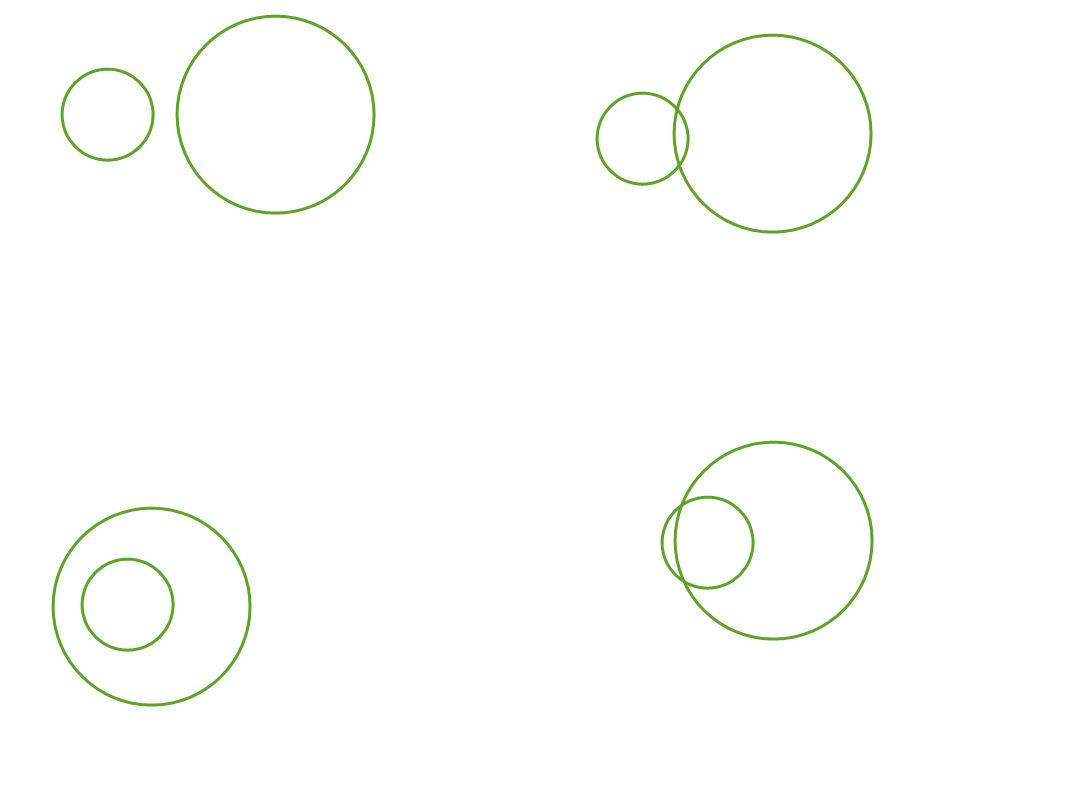
\includegraphics[width=0.4\linewidth]{pic0}
		\caption{}
		\label{fig:pic0}
	\end{figure}
	我们可能更关心第二,三种情况,如下图所示:
	\begin{figure}
		\centering
		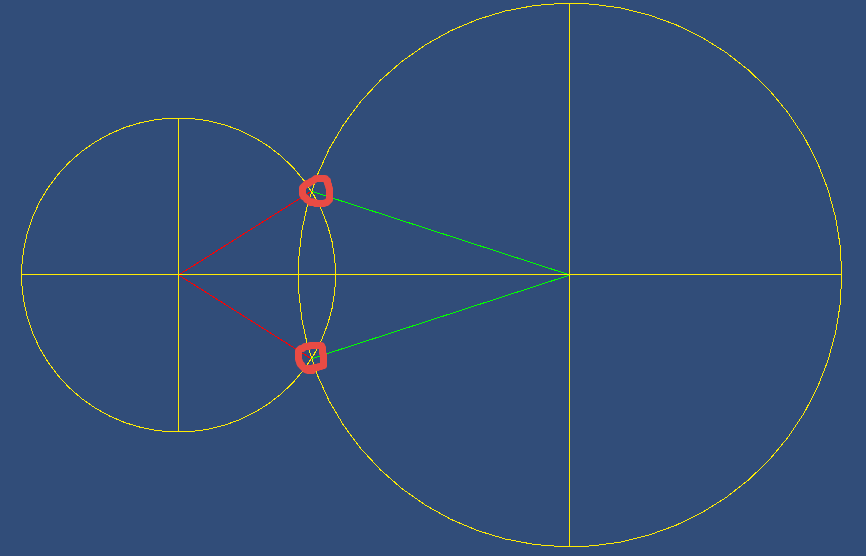
\includegraphics[width=0.7\linewidth]{pic1}
		\caption{}
		\label{fig:pic1}
	\end{figure}
	图中用红笔标记的两个点为我们要求的点:
	\begin{figure}
		\centering
		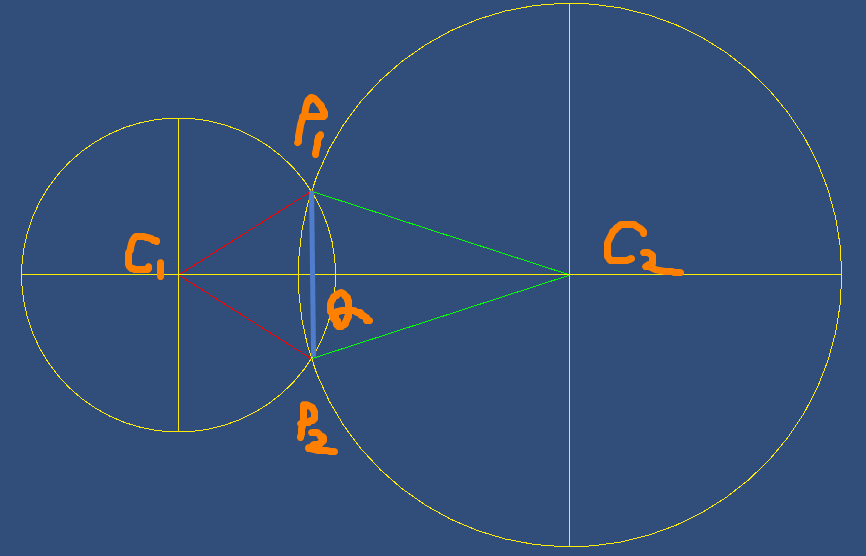
\includegraphics[width=0.7\linewidth]{pic2}
		\caption{}
		\label{fig:pic2}
	\end{figure}
\begin{figure}
	\centering
	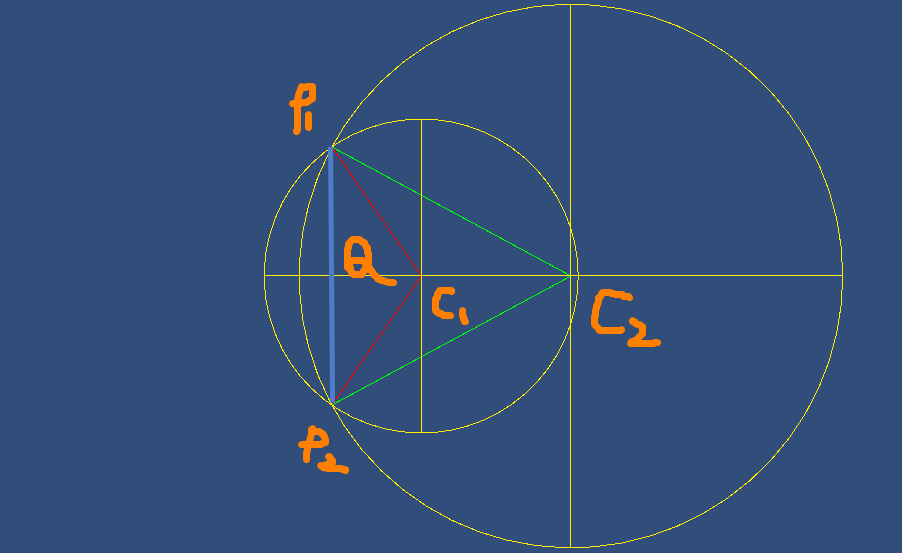
\includegraphics[width=0.5\linewidth]{pic3}
	\caption{}
	\label{fig:pic3}
\end{figure}

	实际上,我们只需要算$P_1$,$P_2$便同理可得,那我们就开始算P1吧,首先有方程:
	\begin{eqnarray}
	\vec{P_1} = \vec{C_1}+\vec{C_1Q}+\vec{QP_1}\\
	\vec{P_1Q}=\vec{QP_2}\\
	\end{eqnarray}\\
	我们甚至可以证明直线$C_1C_2$是图形的对称轴。设\angle$P_1C_1Q$为$\alpha$,我们有方程:
	\begin{eqnarray}
	\arrowvert{C_1Q}\arrowvert = \arrowvert{C_1P_1}\arrowvert\cos\alpha\\
	\cos\alpha=\frac{\arrowvert{C_1P_1}\arrowvert^2+\arrowvert{C_1C_2}\arrowvert^2-\arrowvert{P_1C_2}\arrowvert^2}{2*\arrowvert{C_1P_1}\arrowvert*\arrowvert{C_1C_2}\arrowvert} 
	\end{eqnarray}
	结合$(4)$和$(5)$,我们可以计算出$C_1Q$的长度:
	\begin{eqnarray}
		\arrowvert{C_1Q}\arrowvert=\frac{\arrowvert{C_1P_1}\arrowvert^2+\arrowvert{C_1C_2}\arrowvert^2-\arrowvert{P_1C_2}\arrowvert^2}{2*\arrowvert{C_1C_2}\arrowvert} 
	\end{eqnarray}
	注意,上式$C_1Q$的长度有正负之分,理由看图4就知道了,接下来,我们根据毕式定理得到$P_1Q$的长度,然后只需求出$\vec{C_1C_2}$的normalized向量,记为$\vec{Norm(C_1C_2)}$,我们有:
	\begin{eqnarray}
	\vec{C_1Q}=\vec{C_1}+\arrowvert{C_1Q}\arrowvert*Norm(\vec{C_1C_2})
	\end{eqnarray}
	也就是:
	\begin{eqnarray}
	\vec{C_1Q}=\vec{C_1}+\frac{\arrowvert{C_1P_1}\arrowvert^2+\arrowvert{C_1C_2}\arrowvert^2-\arrowvert{P_1C_2}\arrowvert^2}{2*\vec{C_1C_2}^2} *\vec{C_1C_2}
	\end{eqnarray}
	方程$(7)$是适用于图3,图4这两种情况的,你能看出来吗?
\end{document}
